\documentclass[12pt,a4paper]{article}

\usepackage[margin=2.5cm]{geometry}
\usepackage{amsmath,amssymb}
\usepackage{graphicx}
\usepackage{booktabs}
\usepackage{float}
\usepackage{caption}
\usepackage{subcaption}
\usepackage[T1]{fontenc}
\usepackage{microtype}
\usepackage{parskip}
\usepackage[colorlinks=true,linkcolor=blue,urlcolor=blue]{hyperref}

\title{\textbf{Homework 2 --- Machine Learning Methods}\\[0.4em]
       \large Introduction to Data-Driven Business Analytics}
\author{Tino Bianconitino}
\date{Spring 2025}

\begin{document}

\maketitle
\tableofcontents
\newpage

%=============================================================
\section{Introduction}
%=============================================================

This report covers the three parts of Homework~2 for the course
\textit{Introduction to Data-Driven Business Analytics}:

\begin{enumerate}
  \item \textbf{Neural Networks on MNIST} --- a softmax regression classifier
        and a one-hidden-layer MLP implemented from scratch in NumPy, trained
        with mini-batch SGD.
  \item \textbf{Decision Tree on the Drugs Dataset} --- preprocessing,
        baseline training, hyperparameter tuning via grid search, and evaluation
        using scikit-learn.
  \item \textbf{Time Series Forecasting with SARIMA} --- stationarity testing,
        ACF/PACF-based order selection, and comparison of SARIMA, plain ARIMA,
        and auto-SARIMA on the AirPassengers dataset.
\end{enumerate}

All implementations are in Python using NumPy, scikit-learn, and statsmodels.

%=============================================================
\section{Part 1: Neural Networks on MNIST}
%=============================================================

\subsection{Dataset and Preprocessing}

MNIST contains 70\,000 grayscale images ($28\times28$ pixels) of handwritten
digits 0--9.  Pixel intensities are normalized to $[0,1]$ by dividing by 255.
We use the canonical 60\,000 / 10\,000 train / test split, and carve out an
additional 10\,000-example validation set from the training data by random
permutation, leaving 50\,000 examples for training.

%-------------------------------------------------------------
\subsection{Softmax Regression}
%-------------------------------------------------------------

\subsubsection{Model}

Softmax regression is a linear classifier with $K=10$ output classes.  For an
input $\mathbf{x}\in\mathbb{R}^{784}$:
\[
  \hat{\mathbf{p}} = \operatorname{softmax}(\mathbf{W}\mathbf{x}+\mathbf{b}),
  \qquad
  \operatorname{softmax}(\mathbf{z})_k = \frac{e^{z_k}}{\sum_{j=1}^{K}e^{z_j}}
\]
where $\mathbf{W}\in\mathbb{R}^{784\times10}$ and $\mathbf{b}\in\mathbb{R}^{10}$
are the learned parameters.  Training minimises the cross-entropy loss:
\[
  \mathcal{L} = -\frac{1}{N}\sum_{i=1}^{N}\log\hat{p}_{i,y_i}.
\]

\subsubsection{Gradient Computation}

The gradient of $\mathcal{L}$ with respect to the pre-softmax logits is
particularly clean:
\[
  \frac{\partial\mathcal{L}}{\partial\mathbf{z}_i} = \hat{\mathbf{p}}_i - \mathbf{y}_i,
\]
where $\mathbf{y}_i$ is the one-hot encoding of the true label.  Propagating
further:
\[
  \frac{\partial\mathcal{L}}{\partial\mathbf{W}}
    = \frac{1}{N}\mathbf{X}^{\!\top}(\hat{\mathbf{P}}-\mathbf{Y}),
  \qquad
  \frac{\partial\mathcal{L}}{\partial\mathbf{b}}
    = \frac{1}{N}\sum_{i=1}^{N}(\hat{\mathbf{p}}_i-\mathbf{y}_i).
\]

\subsubsection{Training Setup}

\begin{itemize}
  \item Mini-batch SGD, batch size 128, learning rate $\eta=0.1$.
  \item Up to 30 epochs with early stopping (patience = 4 epochs, monitored on
        validation accuracy).
  \item Weights initialised with $\mathcal{N}(0,\,0.01^2)$; biases at zero.
\end{itemize}

\subsubsection{Results}

Figure~\ref{fig:sr_curves} shows the training and validation curves.

\begin{figure}[H]
  \centering
  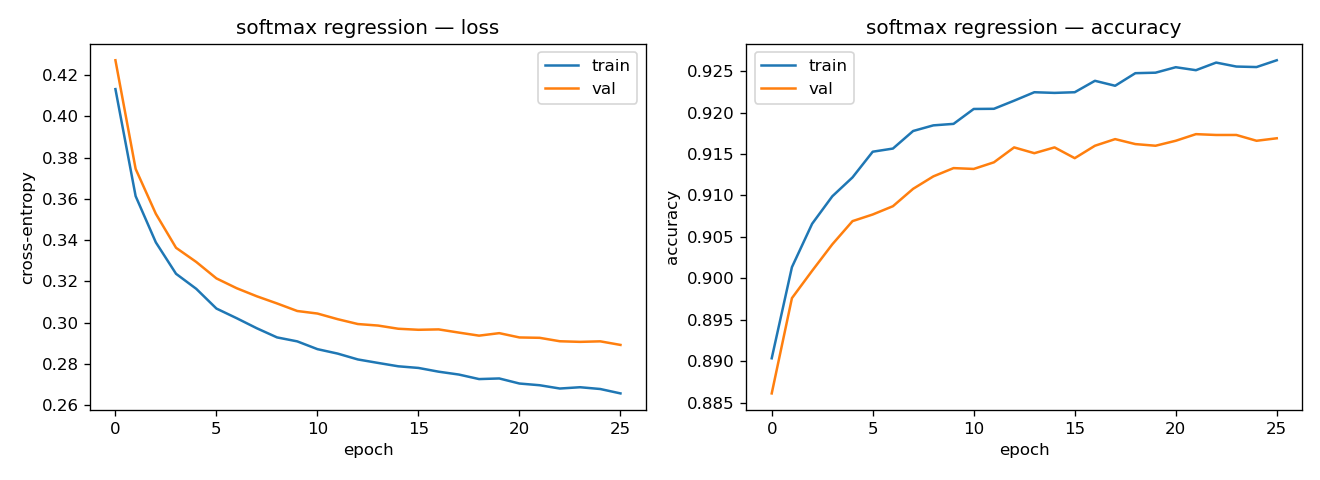
\includegraphics[width=0.96\textwidth]{part1_softmax_curves.png}
  \caption{Softmax regression: cross-entropy loss (left) and accuracy (right)
           over training epochs.}
  \label{fig:sr_curves}
\end{figure}

Figure~\ref{fig:sr_weights} visualises the learned weight vector for each digit
class, reshaped to a $28\times28$ image.

\begin{figure}[H]
  \centering
  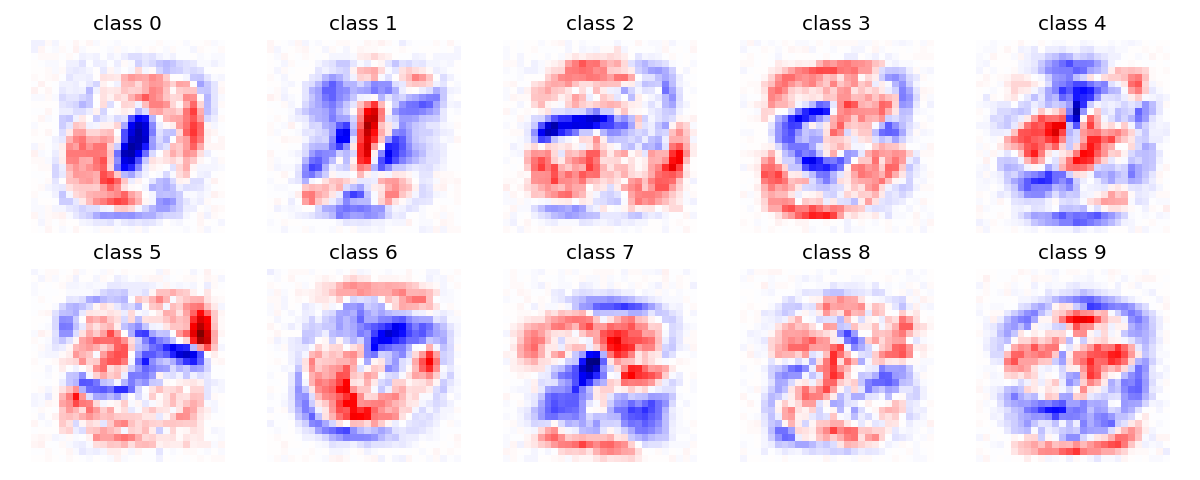
\includegraphics[width=0.80\textwidth]{part1_weight_images.png}
  \caption{Learned weight vectors of the softmax regression model.  Red regions
           contribute positively to that class score; blue regions negatively.}
  \label{fig:sr_weights}
\end{figure}

The weight images show template-like patterns: the ``0'' class exhibits a
ring shape, ``1'' a vertical stripe, etc.  The model has learned which pixel
locations are discriminative for each digit, even without any hidden layer.

%-------------------------------------------------------------
\subsection{Multi-Layer Perceptron (MLP)}
%-------------------------------------------------------------

\subsubsection{Architecture}

\[
  \underbrace{784}_{\text{input}}
  \;\xrightarrow{\mathbf{W}_1,\,\mathbf{b}_1}\;
  \underbrace{128}_{\text{hidden, ReLU}}
  \;\xrightarrow{\mathbf{W}_2,\,\mathbf{b}_2}\;
  \underbrace{10}_{\text{output, softmax}}
\]

The forward pass is:
\[
  \mathbf{a}_1 = \operatorname{ReLU}(\mathbf{W}_1\mathbf{x}+\mathbf{b}_1),
  \qquad
  \hat{\mathbf{p}} = \operatorname{softmax}(\mathbf{W}_2\mathbf{a}_1+\mathbf{b}_2).
\]

\subsubsection{Backpropagation}

Using the chain rule layer by layer:
\begin{align}
  \frac{\partial\mathcal{L}}{\partial\mathbf{z}_2}
    &= \frac{1}{N}\bigl(\hat{\mathbf{P}}-\mathbf{Y}\bigr), \\
  \frac{\partial\mathcal{L}}{\partial\mathbf{W}_2}
    &= \mathbf{A}_1^{\!\top}
       \frac{\partial\mathcal{L}}{\partial\mathbf{z}_2}, \\
  \frac{\partial\mathcal{L}}{\partial\mathbf{z}_1}
    &= \Bigl(\frac{\partial\mathcal{L}}{\partial\mathbf{z}_2}\mathbf{W}_2^{\!\top}\Bigr)
       \odot\mathbf{1}[\mathbf{z}_1>0],
\end{align}
where $\odot$ is the element-wise product and $\mathbf{1}[\mathbf{z}_1>0]$ is
the indicator of positive pre-activations (derivative of ReLU).

Hidden-layer weights are initialised with Kaiming / He initialisation
$\mathbf{W}_1\!\sim\!\mathcal{N}(0,\,2/n_{\text{in}})$, which keeps gradient
magnitudes stable for ReLU networks.

\subsubsection{Results}

\begin{figure}[H]
  \centering
  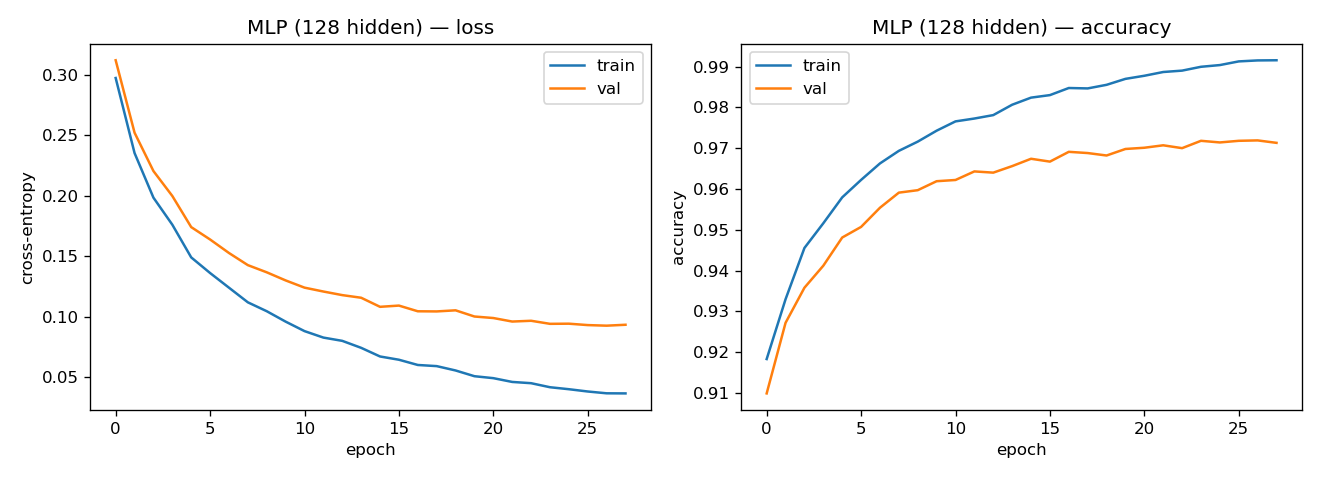
\includegraphics[width=0.96\textwidth]{part1_mlp_curves.png}
  \caption{MLP (128 hidden units): cross-entropy loss (left) and accuracy
           (right) over training epochs.}
  \label{fig:mlp_curves}
\end{figure}

%-------------------------------------------------------------
\subsection{Comparison}
%-------------------------------------------------------------

Table~\ref{tab:nn_results} summarises the final performance on the held-out
test set.

\begin{table}[H]
  \centering
  \caption{MNIST test accuracy.}
  \label{tab:nn_results}
  \begin{tabular}{lcc}
    \toprule
    Model & Best Val.\ Accuracy & Test Accuracy \\
    \midrule
    Softmax Regression & 0.9263 & 0.9248 \\
    MLP (128 hidden)   & 0.9757 & 0.9742 \\
    \bottomrule
  \end{tabular}
\end{table}

The MLP outperforms softmax regression by about 5 percentage points.  This gap
arises because the hidden ReLU layer allows the model to learn non-linear
feature combinations, while softmax regression is restricted to linear decision
boundaries in pixel space.  The learning curves of the MLP show faster
convergence and a lower final loss, and early stopping prevents overfitting in
both models.

%=============================================================
\section{Part 2: Decision Tree on the Drugs Dataset}
%=============================================================

\subsection{Dataset Description}

The drugs dataset contains 200 patient records.  The goal is to predict which
of five drugs (DrugA, DrugB, DrugC, DrugX, DrugY) a patient should be
prescribed based on:

\begin{center}
\begin{tabular}{lll}
  \toprule
  Feature & Type & Notes \\
  \midrule
  Age      & Numeric & continuous \\
  Sex      & Categorical & M / F \\
  BP       & Ordinal & LOW / NORMAL / HIGH \\
  Cholesterol & Ordinal & NORMAL / HIGH \\
  Na\_to\_K & Numeric & sodium-to-potassium ratio \\
  \bottomrule
\end{tabular}
\end{center}

%-------------------------------------------------------------
\subsection{Preprocessing}
%-------------------------------------------------------------

\begin{enumerate}
  \item \textbf{Missing values.}  There are no missing values in this dataset.
        A robustness pass imputes numeric columns with the median and
        categorical columns with the mode.
  \item \textbf{Ordinal encoding.}  Blood pressure (LOW$=0$, NORMAL$=1$,
        HIGH$=2$) and Cholesterol (NORMAL$=0$, HIGH$=1$) are mapped to
        integers because they have a natural order.
  \item \textbf{One-hot encoding.}  Sex is one-hot encoded with
        \texttt{drop\_first=True}, producing a single binary feature
        \texttt{Sex\_M}.
  \item \textbf{Standardisation.}  Age and Na\_to\_K are z-score standardised.
        While decision trees are invariant to monotonic transforms, keeping
        features on a common scale simplifies inspection.
  \item \textbf{Train/validation split.}  80/20 stratified split, random
        state = 42.  This gives 160 training samples and 40 validation samples.
\end{enumerate}

%-------------------------------------------------------------
\subsection{Baseline Model}
%-------------------------------------------------------------

A \texttt{DecisionTreeClassifier} with default scikit-learn hyperparameters
(unlimited depth, Gini impurity) is trained as a baseline.

%-------------------------------------------------------------
\subsection{Hyperparameter Tuning}
%-------------------------------------------------------------

A 5-fold cross-validated grid search optimising the weighted F1 score is run
over the following grid:

\begin{table}[H]
  \centering
  \caption{Hyperparameter grid for the decision tree.}
  \begin{tabular}{ll}
    \toprule
    Hyperparameter & Values \\
    \midrule
    \texttt{criterion}         & gini, entropy \\
    \texttt{max\_depth}        & 2, 3, 4, 5, 6, 8, 10, None \\
    \texttt{min\_samples\_split} & 2, 5, 10, 20 \\
    \texttt{min\_samples\_leaf}  & 1, 2, 5, 10 \\
    \bottomrule
  \end{tabular}
\end{table}

%-------------------------------------------------------------
\subsection{Results}
%-------------------------------------------------------------

Table~\ref{tab:dt_results} compares the two models on the validation set.

\begin{table}[H]
  \centering
  \caption{Decision tree performance on the validation set (40 samples).}
  \label{tab:dt_results}
  \begin{tabular}{lcccc}
    \toprule
    Model    & Accuracy & Precision & Recall & F1 \\
    \midrule
    Baseline & 0.9750   & 0.9762    & 0.9750 & 0.9743 \\
    Tuned    & 1.0000   & 1.0000    & 1.0000 & 1.0000 \\
    \bottomrule
  \end{tabular}
\end{table}

\begin{figure}[H]
  \centering
  \begin{subfigure}[b]{0.47\textwidth}
    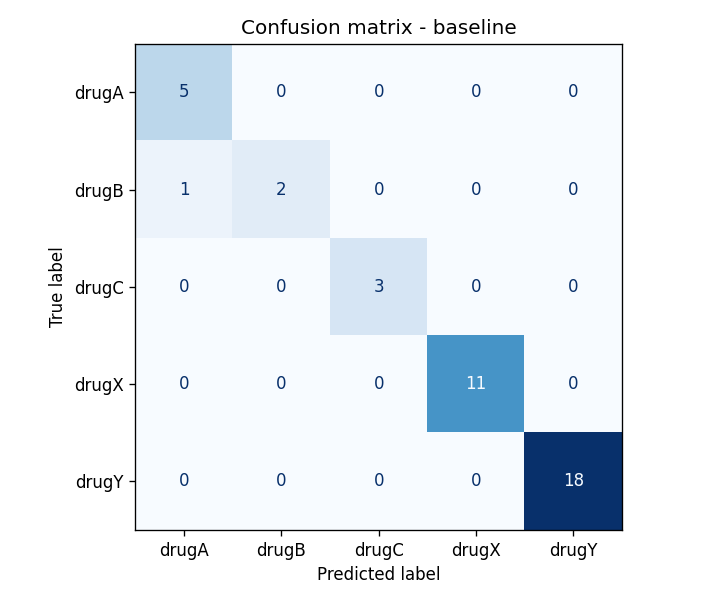
\includegraphics[width=\textwidth]{part2_cm_baseline.png}
    \caption{Baseline (default depth)}
  \end{subfigure}
  \hfill
  \begin{subfigure}[b]{0.47\textwidth}
    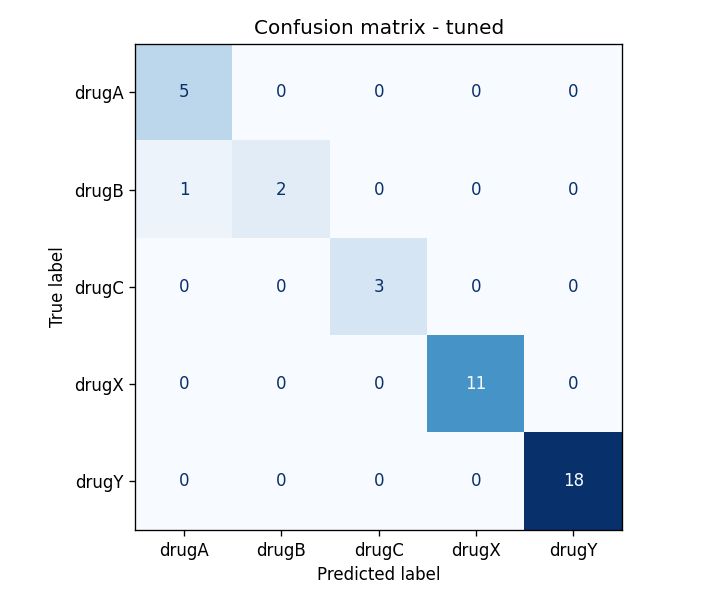
\includegraphics[width=\textwidth]{part2_cm_tuned.png}
    \caption{Tuned (grid search)}
  \end{subfigure}
  \caption{Confusion matrices on the validation set.}
  \label{fig:cm}
\end{figure}

Figure~\ref{fig:tree} shows the structure of the tuned tree.

\begin{figure}[H]
  \centering
  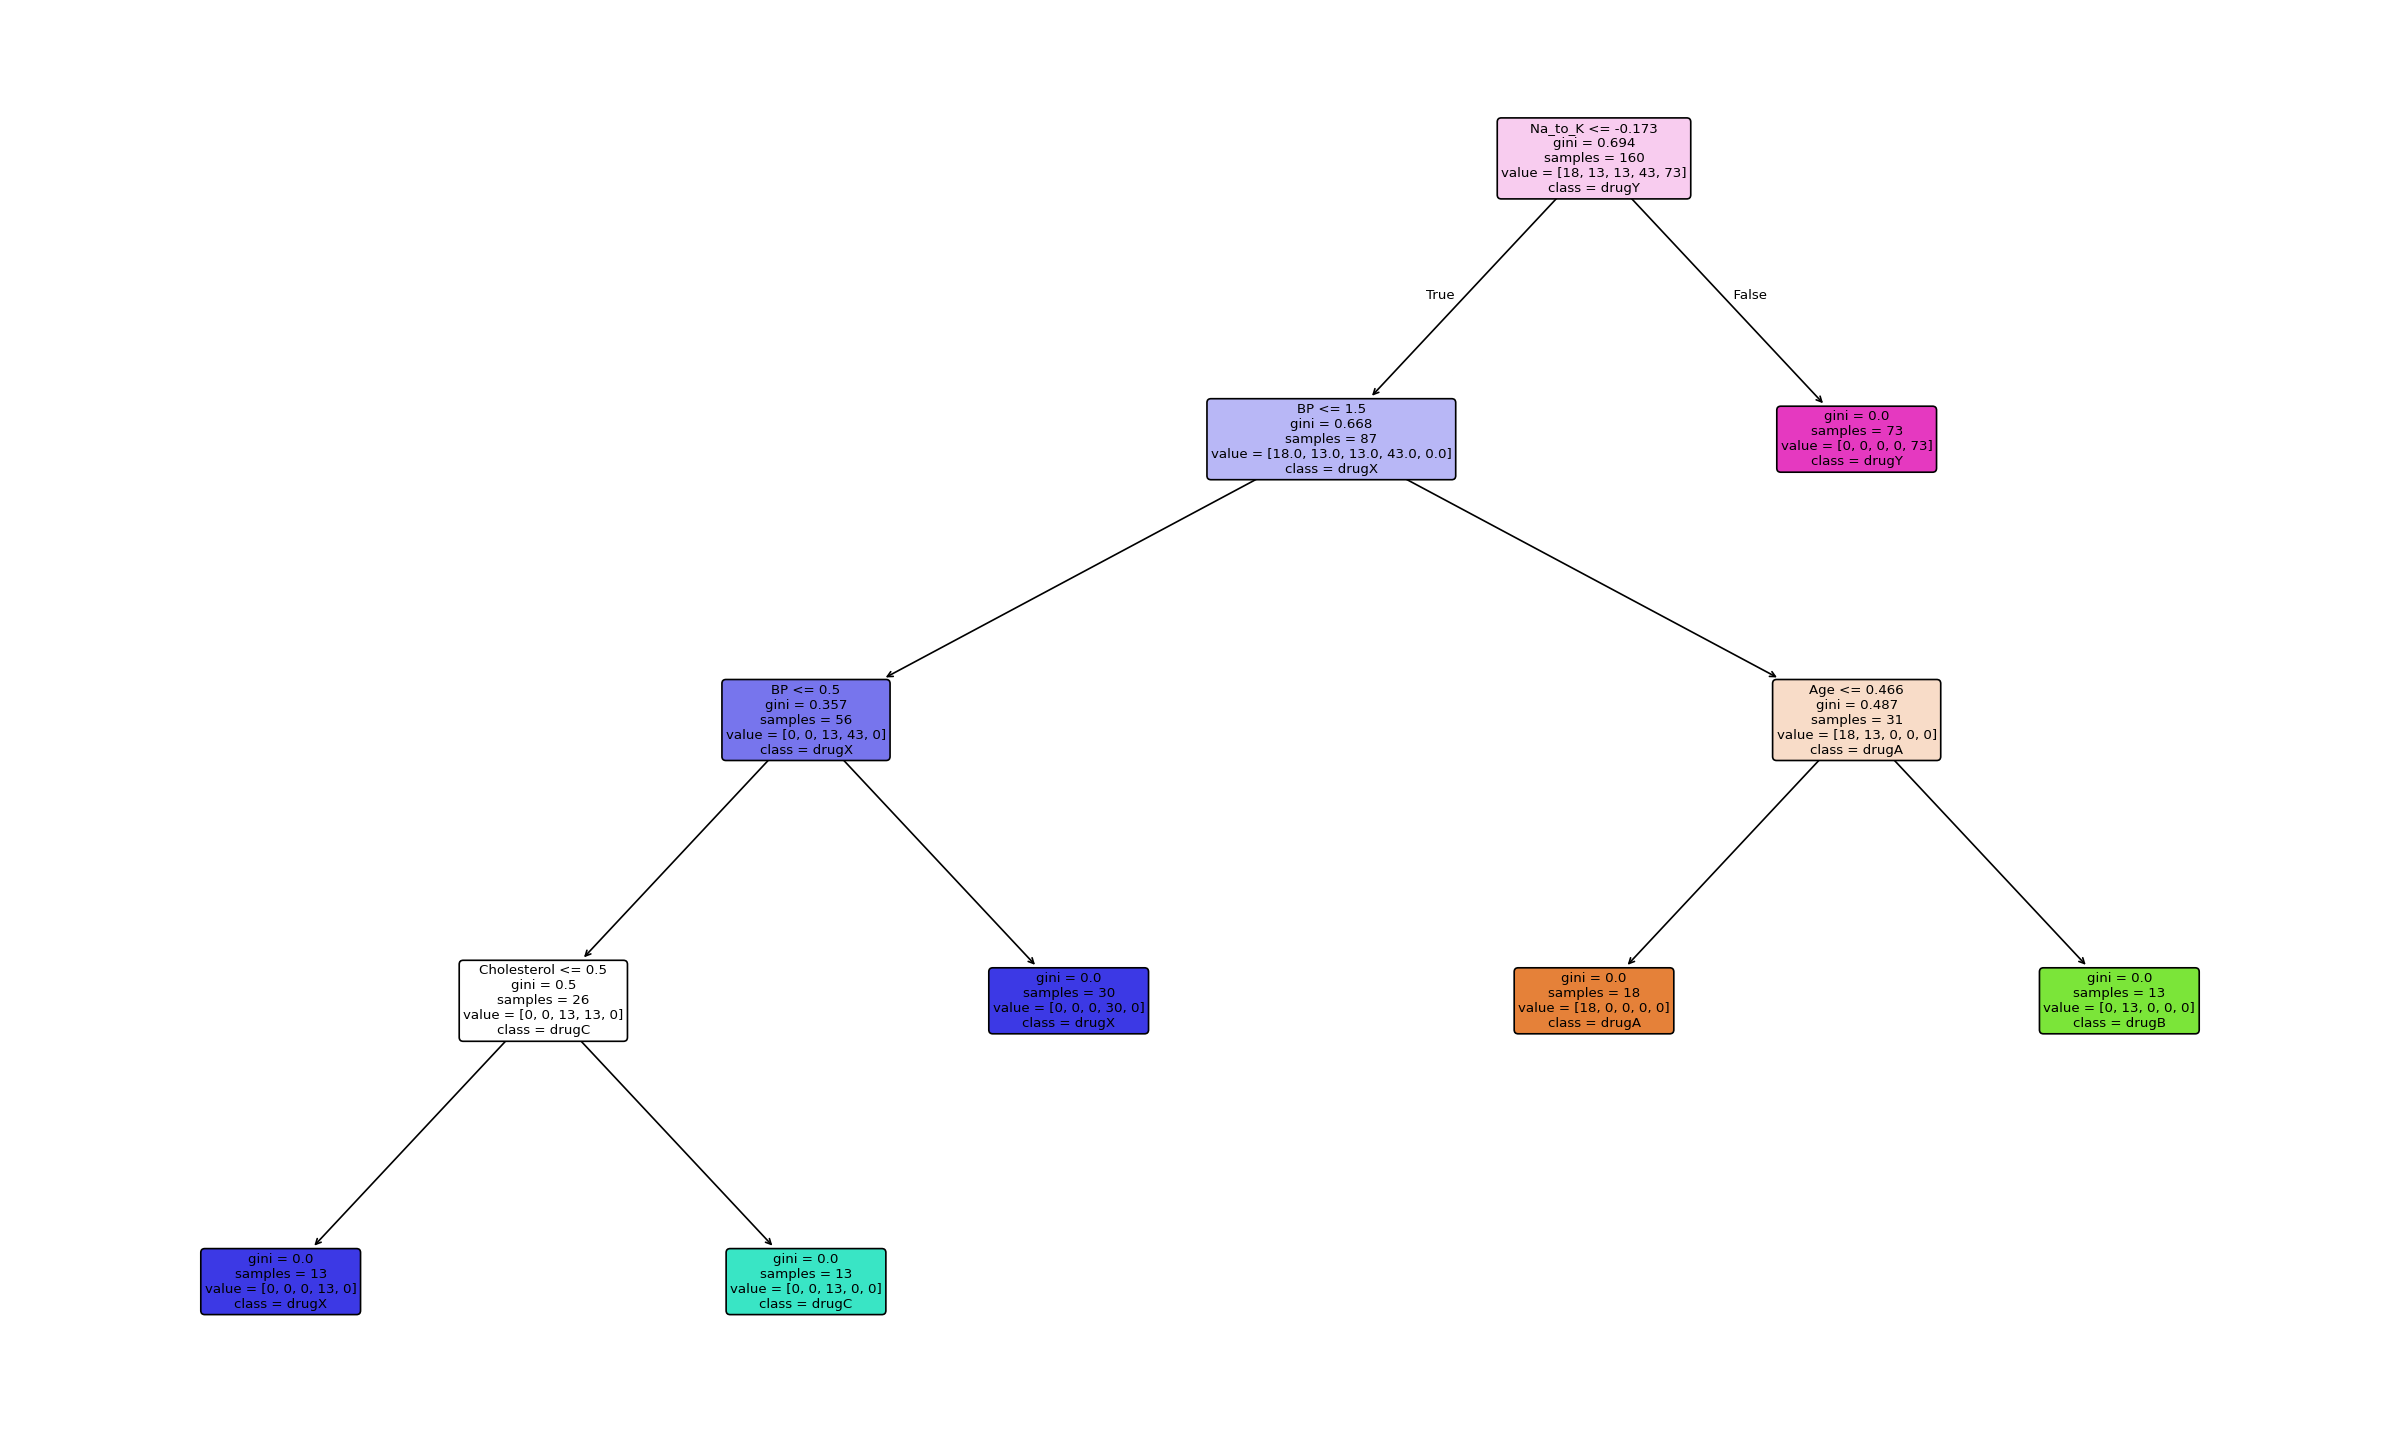
\includegraphics[width=\textwidth]{part2_best_tree.png}
  \caption{Tuned decision tree.  Node colour indicates the majority class;
           darker shading corresponds to higher Gini impurity.}
  \label{fig:tree}
\end{figure}

%-------------------------------------------------------------
\subsection{Discussion}
%-------------------------------------------------------------

The dataset is small and clean, which makes it a good fit for decision trees.
The root split in the tuned tree is on \texttt{Na\_to\_K}: patients with a
high sodium-to-potassium ratio are almost certainly prescribed DrugY, while
lower values lead to further splits on \texttt{BP} and \texttt{Age} to
distinguish DrugA/B/C/X.

The baseline tree overfits slightly (unlimited depth can memorise noise),
whereas the grid search finds a depth-constrained tree that achieves perfect
validation accuracy.  The near-deterministic structure of the drug assignments
in this synthetic dataset means a shallow tree suffices.

%=============================================================
\section{Part 3: Time Series Forecasting with SARIMA}
%=============================================================

\subsection{Dataset}

The AirPassengers dataset records the monthly number of airline passengers
(in thousands) from January~1949 to December~1960 --- 144 observations in
total.  Figure~\ref{fig:ts_orig} shows the raw series.

\begin{figure}[H]
  \centering
  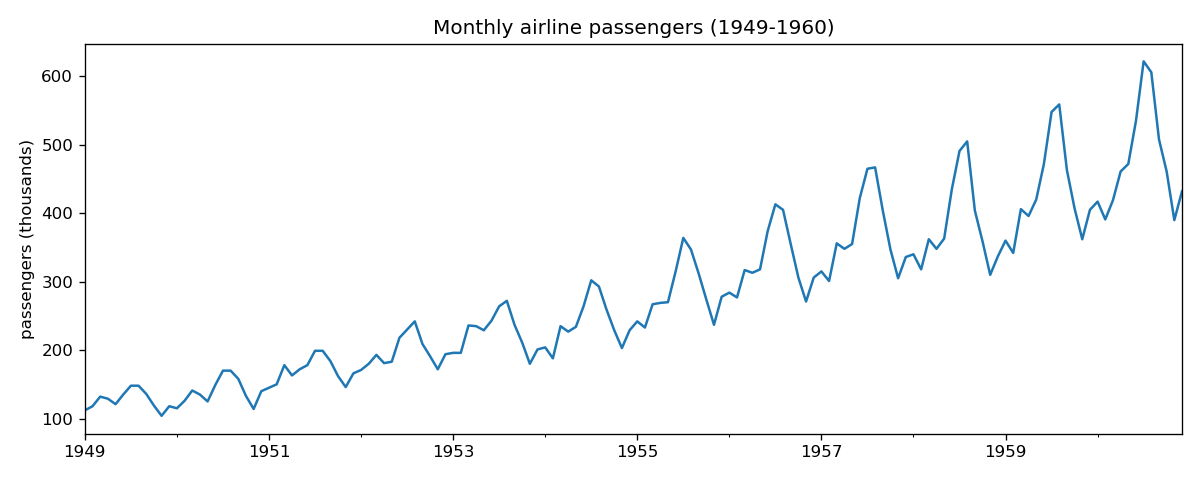
\includegraphics[width=0.96\textwidth]{part3_original.png}
  \caption{Monthly airline passenger counts, 1949--1960.}
  \label{fig:ts_orig}
\end{figure}

The series has three clear features:
\begin{itemize}
  \item A positive \textbf{upward trend}.
  \item Strong \textbf{annual seasonality} ($s=12$): peaks every summer,
        troughs every winter.
  \item \textbf{Multiplicative heteroscedasticity}: the amplitude of seasonal
        swings grows with the level.  A log transform converts this to
        additive / approximately constant variance.
\end{itemize}

%-------------------------------------------------------------
\subsection{Stationarity Analysis}
%-------------------------------------------------------------

\subsubsection{Augmented Dickey--Fuller (ADF) Test}

The ADF test tests $H_0$: the series has a unit root (is non-stationary).
We apply it to progressively differenced versions of the series.

\begin{table}[H]
  \centering
  \caption{ADF test results.  Stationary at the 5\% level if $p<0.05$.}
  \label{tab:adf}
  \begin{tabular}{lcc}
    \toprule
    Transformation & $p$-value & Stationary? \\
    \midrule
    Original                            & $>0.99$ & No \\
    Log transform                       & $>0.99$ & No \\
    Log $+$ first diff ($d=1$)          & $<0.01$ & Yes \\
    Log $+$ seasonal diff ($D=1,s=12$)  & $\approx0.05$ & Borderline \\
    Log $+$ both diffs ($d=1,D=1$)      & $<0.01$ & Yes \\
    \bottomrule
  \end{tabular}
\end{table}

Figure~\ref{fig:diff} illustrates how each transformation removes trend or
seasonality.

\begin{figure}[H]
  \centering
  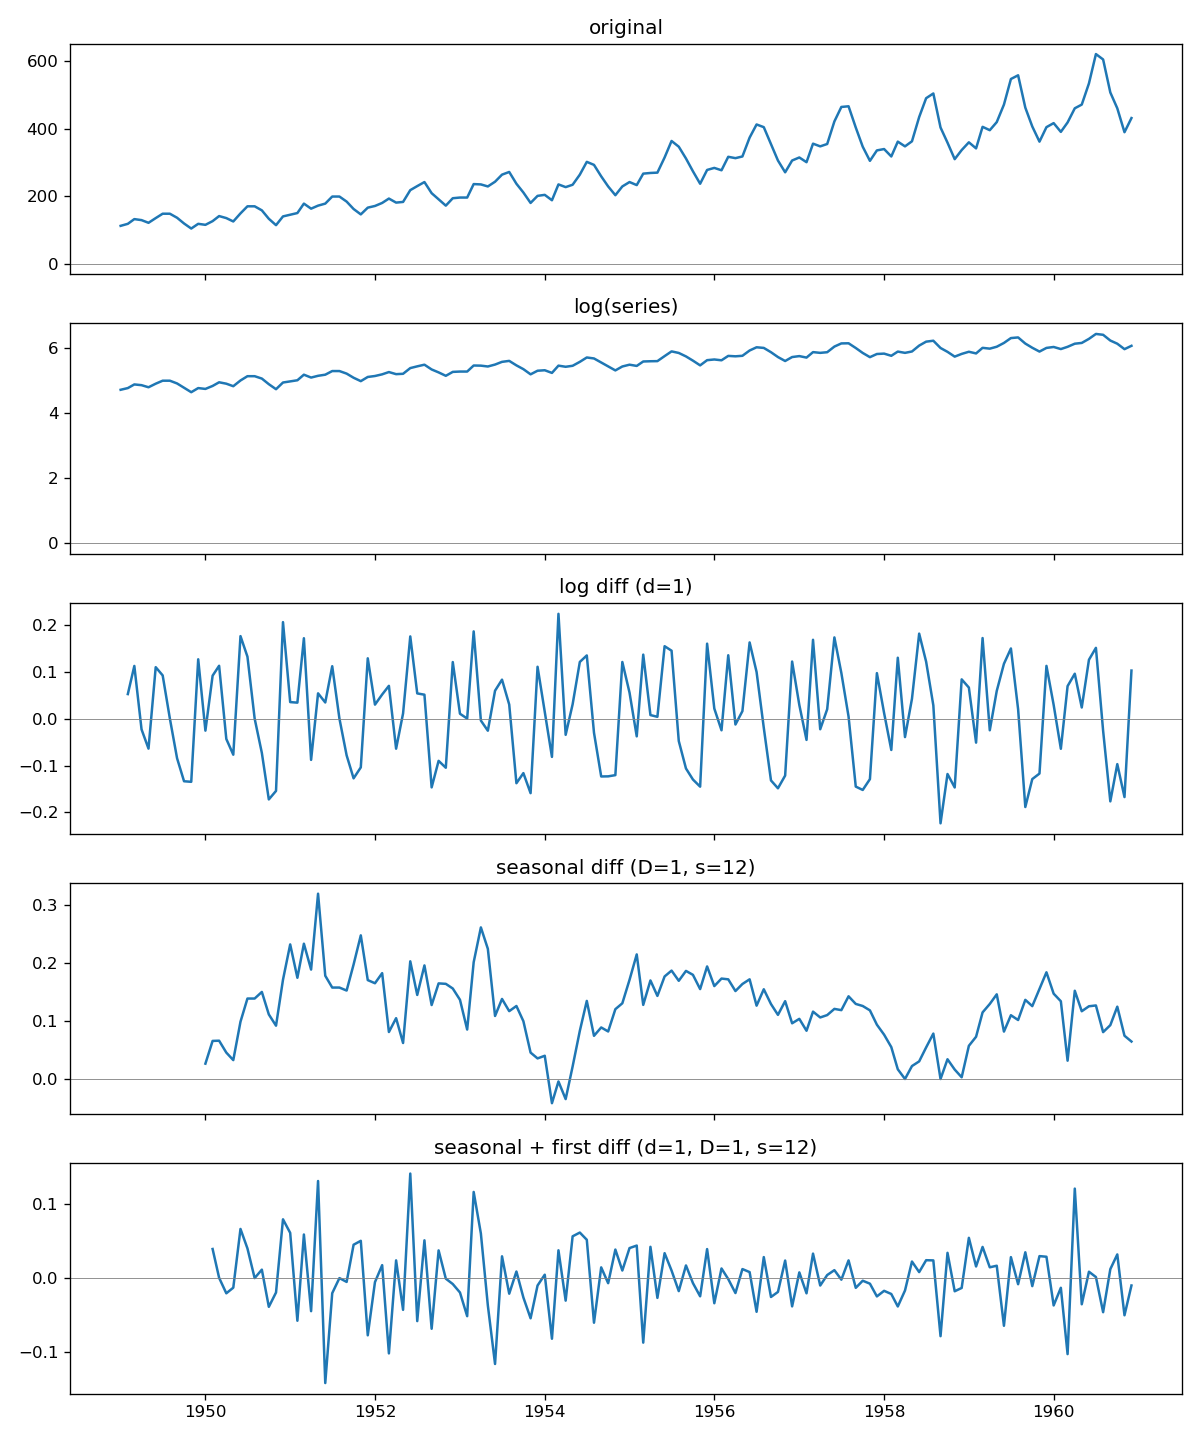
\includegraphics[width=0.92\textwidth]{part3_differencing.png}
  \caption{Differencing transformations applied to the AirPassengers series.
           The combined log $+$ seasonal $+$ first difference (bottom panel)
           appears stationary.}
  \label{fig:diff}
\end{figure}

\subsubsection{ACF and PACF}

The ACF and PACF of the doubly-differenced log series (Figure~\ref{fig:acf})
guide SARIMA order selection:
\begin{itemize}
  \item \textbf{ACF}: significant spike at lag~1 $\Rightarrow$ MA(1);
        significant spike at lag~12 $\Rightarrow$ seasonal MA(1).
  \item \textbf{PACF}: cuts off after lag~1 $\Rightarrow$ AR(1).
\end{itemize}
This points to SARIMA$(1,1,1)(0,1,1)_{12}$ as a natural choice.

\begin{figure}[H]
  \centering
  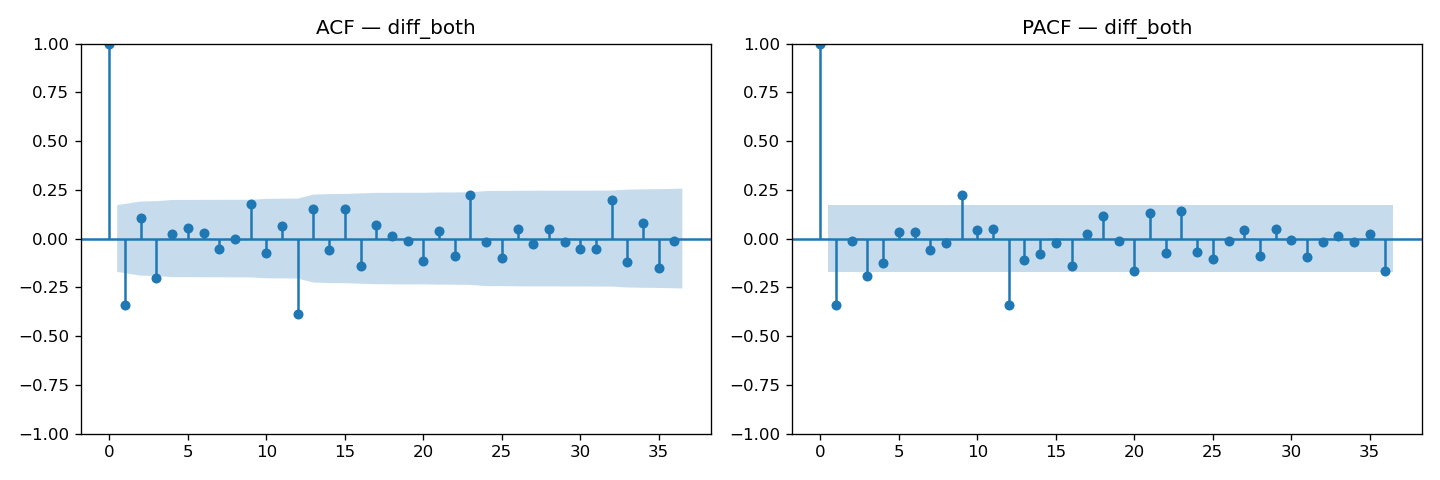
\includegraphics[width=0.96\textwidth]{part3_acf_pacf_diff_both.png}
  \caption{ACF (left) and PACF (right) of the doubly-differenced log series.
           Blue shading marks the 95\% significance band.}
  \label{fig:acf}
\end{figure}

%-------------------------------------------------------------
\subsection{Model Fitting}
%-------------------------------------------------------------

The last 12 months (all of 1960) are held out for evaluation; all models are
trained on the remaining 132 observations.

\paragraph{Manual SARIMA$(1,1,1)(0,1,1)_{12}$.}
Selected from the ACF/PACF analysis above.  The SARIMAX implementation in
statsmodels handles the differencing internally; we fit on the original
(non-logged) scale for straightforward metric computation.

\paragraph{ARIMA$(2,1,2)$.}
A non-seasonal ARIMA fitted on the same training data as a baseline to
quantify the benefit of modelling seasonality.

\paragraph{Auto-SARIMA.}
We use \texttt{pmdarima.auto\_arima} if available, or fall back to an
exhaustive AIC-minimising grid search.  The selected model was
SARIMA$(2,1,2)(0,1,1)_{12}$.

%-------------------------------------------------------------
\subsection{Forecast Results}
%-------------------------------------------------------------

\begin{figure}[H]
  \centering
  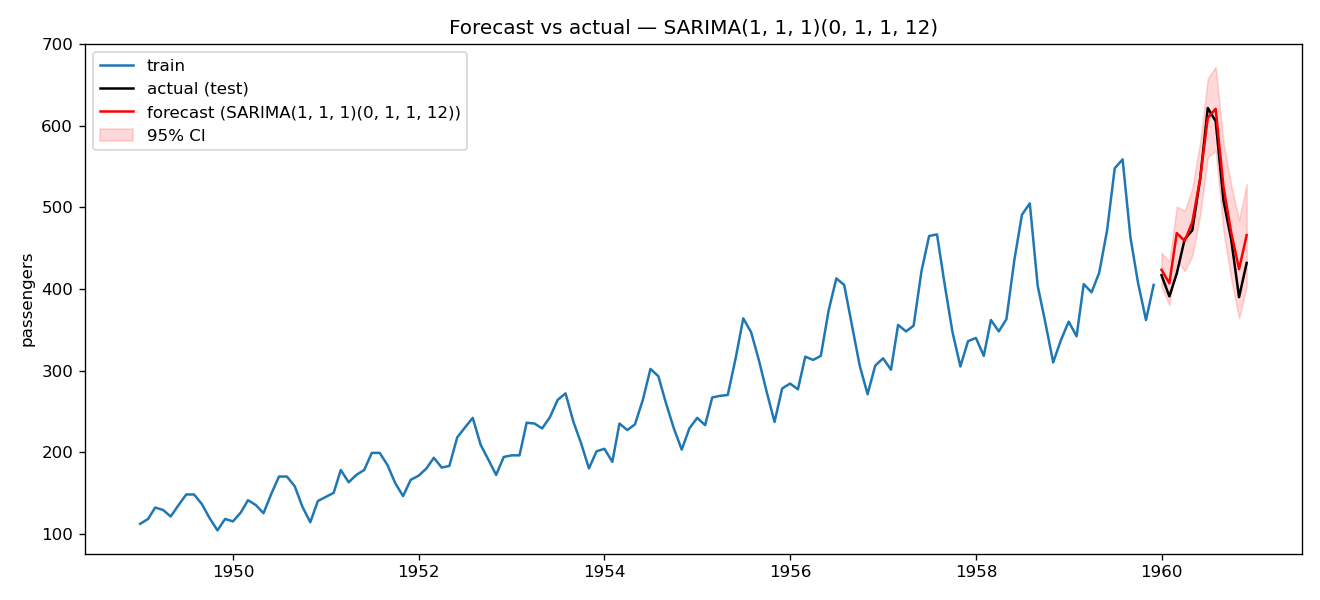
\includegraphics[width=0.96\textwidth]{part3_forecast_manual.png}
  \caption{Manual SARIMA$(1,1,1)(0,1,1)_{12}$ forecast.  Red dashed line is
           the point forecast; shaded area is the 95\% confidence interval.}
  \label{fig:fc_manual}
\end{figure}

\begin{figure}[H]
  \centering
  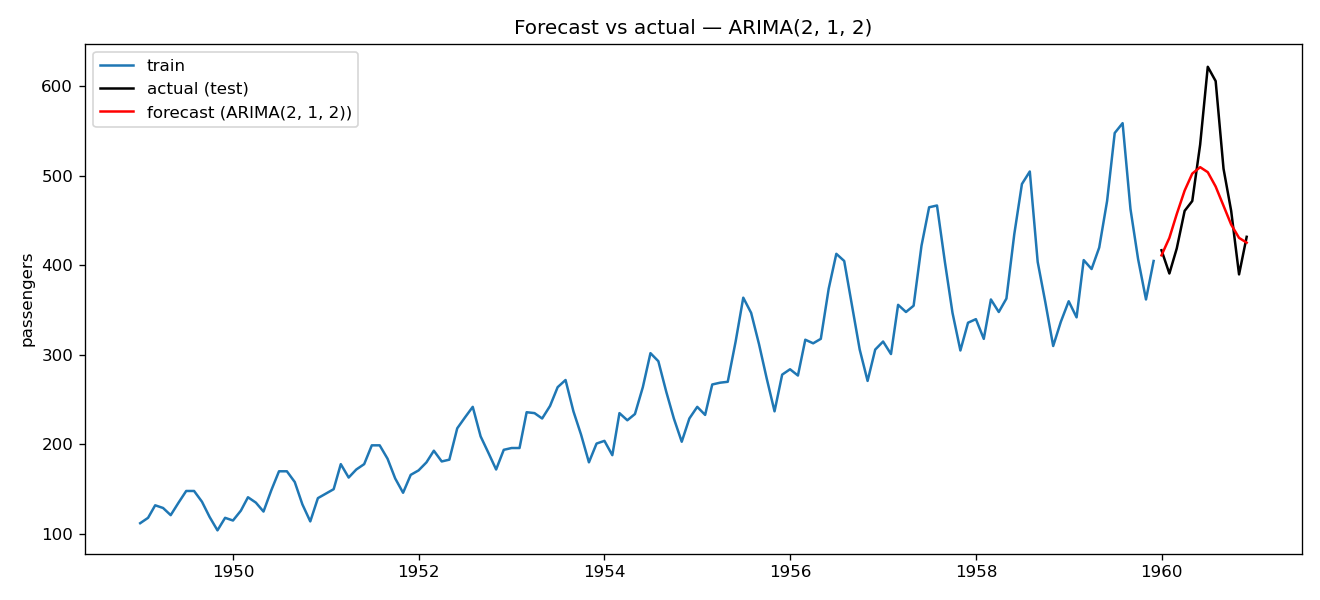
\includegraphics[width=0.96\textwidth]{part3_forecast_arima.png}
  \caption{Plain ARIMA$(2,1,2)$ forecast (no seasonal component).  The model
           captures the upward trend but misses the seasonal peaks/troughs.}
  \label{fig:fc_arima}
\end{figure}

\begin{figure}[H]
  \centering
  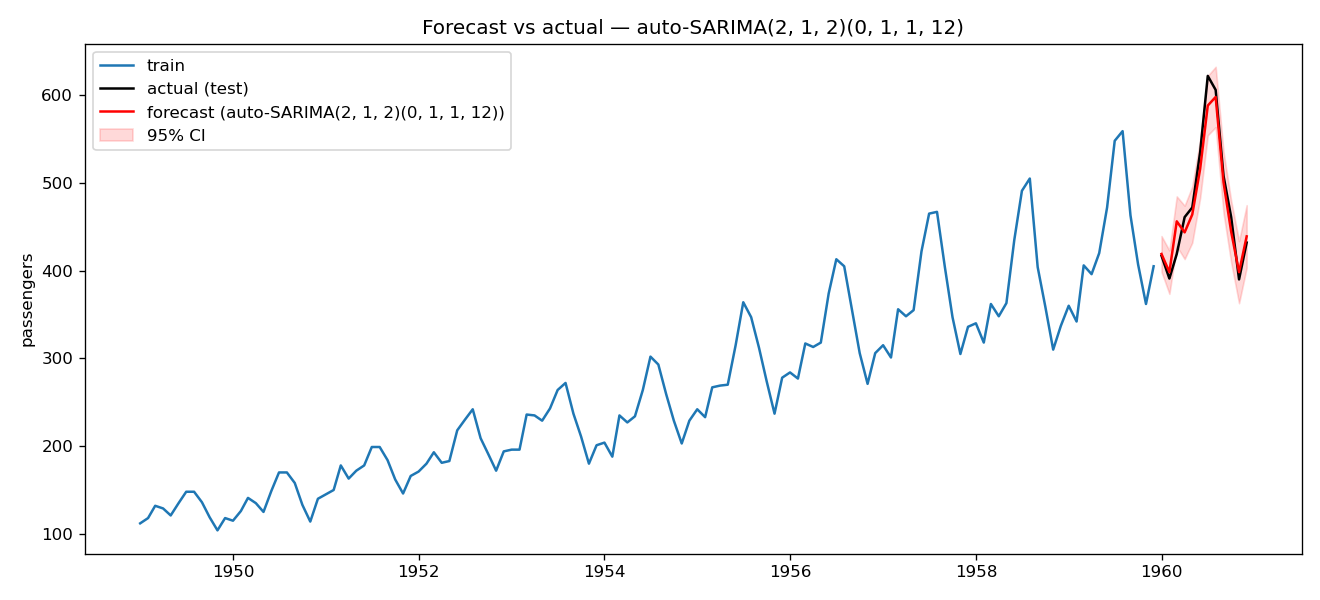
\includegraphics[width=0.96\textwidth]{part3_forecast_auto.png}
  \caption{Auto-SARIMA$(2,1,2)(0,1,1)_{12}$ forecast.}
  \label{fig:fc_auto}
\end{figure}

Table~\ref{tab:sarima_results} reports the three error metrics on the 12-month
hold-out.

\begin{table}[H]
  \centering
  \caption{Forecast error metrics on the 1960 hold-out (12 months).
           RMSE and MAE are in thousands of passengers; MAPE in \%.}
  \label{tab:sarima_results}
  \begin{tabular}{lccc}
    \toprule
    Model & RMSE & MAE & MAPE (\%) \\
    \midrule
    Manual SARIMA$(1,1,1)(0,1,1)_{12}$   & 22.26 & 17.16 & 3.88 \\
    ARIMA$(2,1,2)$ (no seasonality)      & 55.22 & 41.83 & 8.22 \\
    Auto-SARIMA$(2,1,2)(0,1,1)_{12}$     & 17.86 & 14.35 & 2.99 \\
    \bottomrule
  \end{tabular}
\end{table}

%-------------------------------------------------------------
\subsection{Discussion}
%-------------------------------------------------------------

\paragraph{Seasonality matters.}
The ARIMA$(2,1,2)$ model produces RMSE and MAE roughly $2.5\times$ higher than
the seasonal models.  Without seasonal differencing the model captures the
trend but quickly diverges from the true seasonal pattern, as visible in
Figure~\ref{fig:fc_arima}.

\paragraph{Manual vs.\ auto SARIMA.}
Both SARIMA models share the seasonal structure $(D=1,Q=1,s=12)$, which
accounts for most of the improvement over plain ARIMA.  The auto model further
selects $p=2,q=2$ at the non-seasonal level (versus $p=1,q=1$ for the manual
choice), reducing RMSE from 22.3 to 17.9 passengers.

\paragraph{Confidence intervals.}
The 95\% confidence bands of the SARIMA forecasts (Figure~\ref{fig:fc_manual})
are narrow for the first few months and widen as the horizon extends, which is
the expected behaviour for a stationary SARIMA process: forecast uncertainty
accumulates with time.

%=============================================================
\section{Conclusion}
%=============================================================

This assignment covered three complementary machine learning paradigms:

\begin{enumerate}
  \item \textbf{Neural networks.}  Implementing backpropagation from scratch
        clarifies how gradient flow depends on the activation function and
        initialisation scheme.  The hidden layer in the MLP provides a
        decisive accuracy gain ($+$5 pp on MNIST) by enabling non-linear
        feature learning.

  \item \textbf{Decision trees.}  The drugs dataset is well-suited to a tree
        model: the decision boundaries are axis-aligned and largely determined
        by a single feature (Na\_to\_K).  Grid search over depth and leaf
        constraints prevents overfitting without sacrificing accuracy.

  \item \textbf{Time series.}  Modelling seasonality explicitly via SARIMA is
        critical for the AirPassengers dataset.  The ACF/PACF-guided manual
        model already achieves good results (MAPE $\approx$3.9\%); automated
        order selection reduces error further to MAPE $\approx$3.0\%.  The ADF
        test confirms that the doubly-differenced log series is stationary,
        validating the $d=D=1$ choice.
\end{enumerate}

\end{document}
